%%%%%%%%%%%%%%%%%%%%%%%%%%%%%%%%%%%%%%%%%
% Medium Length Professional CV
% LaTeX Template
% Version 2.0 (8/5/13)
%
% This template has been downloaded from:
% http://www.LaTeXTemplates.com
%
% Original author:
% Trey Hunner (http://www.treyhunner.com/)
%
% Important note:
% This template requires the resume.cls file to be in the same directory as the
% .tex file. The resume.cls file provides the resume style used for structuring the
% document.
%
%%%%%%%%%%%%%%%%%%%%%%%%%%%%%%%%%%%%%%%%%

%----------------------------------------------------------------------------------------
%	PACKAGES AND OTHER DOCUMENT CONFIGURATIONS
%----------------------------------------------------------------------------------------

\documentclass{resume} % Use the custom resume.cls style
\usepackage[utf8]{inputenc}   
\usepackage[left=0.75in,top=0.6in,right=0.75in,bottom=0.6in]{geometry} % Document margins
 \usepackage{comment}
 \usepackage[absolute,showboxes]{textpos}
\usepackage{graphicx}
\usepackage{color}
\usepackage{eso-pic}



\name{Curriculum Vitae} % Your name

%\address{Brinellvägen 23, MSE/KTH, 100 44 Stockholm, Sweden} % Your address
%\address{+46707808642 \\ Rongzhen.Chen@mse.kth.se} % Your phone number and email
%\address{Date of Birth: 04 August, 1983} % Your address

%\usepackage{fancyhdr}
%\pagestyle{fancy}

\newcommand\BackgroundPic{
\put(450,570){
\parbox[t]{\textwidth}{
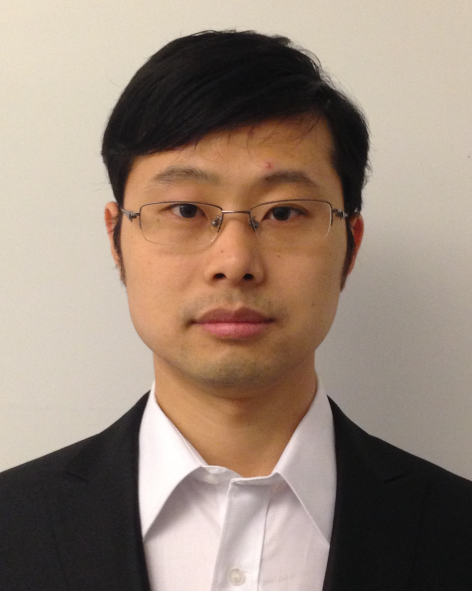
\includegraphics[width=3cm]{myself3}
}
}
}

%\newcommand\BackgroundPic{
%\put(450,550){
%\parbox[t]{\textwidth}{
%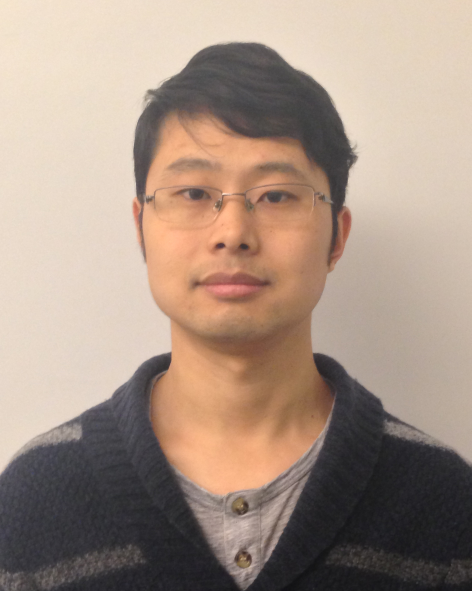
\includegraphics[width=3cm]{myself}
%}
%}
%}


\begin{document}

%----------------------------------------------------------------------------------------
%	EDUCATION SECTION
%----------------------------------------------------------------------------------------

%\begin{textblock}{14}(11,2.1)
%  
\includegraphics[width=4.22cm]{kth}
% \end{textblock}

\AddToShipoutPicture*{\BackgroundPic}

%\rfoot{Kungliga Tekniska högskolan, Brinnellvägen 23, SE-100 44 Stockholm. Tel: +46 (0)70 780 86 42. E-post: Rongzhen.Chen@mse.kth.se}
\begin{rSection}{PERSONAL DETAILS}
 {\bf Name: } \hspace*{14mm} Rongzhen Chen \\
 {\bf Gender: } \hspace*{11mm} Male \\
 {\bf Date of Birth: } August 04, 1983 \\
 {\bf Address: } \hspace*{9.3mm} Arnljot Gellines vei 31 B55, Oslo \\
 {\bf Phone: } \hspace*{12.7mm}  +46 (0) 70 780 86 42  \\
 {\bf Email: } \hspace*{14mm}  Rongzhen.Chen@mse.kth.se \\ 
 

 
\end{rSection}

%\vspace*{1\baselineskip}

\begin{rSection}{EDUCATION AND RESEARCH}
{\bf University of Oslo, Norway} \hfill {Apr. 2016 -- May 2017} \\ 
Researcher at Centre for Materials Science and Nanotechnology.

%Projects: First-Principles Study of Electronic and Optical Properties \\ \hspace*{15.5mm} of Copper-Based Chalcogenide Photovoltaic Materials.

{\bf KTH Royal Institute of Technology, Sweden} \hfill { Sept. 2009 -- May 2017} \\ 
PhD Candidate at Department of Materials Science and Engineering.

%Projects: First-Principles Study of Electronic and Optical Properties \\ \hspace*{15.5mm} of Copper-Based Chalcogenide Photovoltaic Materials.
Projects: First-Principles Study of Copper-Based Chalcogenide Photovoltaic Materials.

Licentiate of Engineering awarded on March 6th, 2015.\\
PhD dissertation defense is expected on May, 2017.

{\bf Northeastern University, P. R. China} \hfill { Sept. 2008 -- July 2009} \\ 
PhD Candidate at College of Information Science and Engineering (Incomplete).

{\bf Northeastern University, P. R. China} \hfill { Sept. 2006 -- July 2008} \\ 
Master of Science at College of Information Science and Engineering. 

%Courses: Java, Matrix Analysis, Equation of Mathematical Physics. \\
Thesis: ANSYS-based Simulations in the Process of Continuous Casting.

{\bf Shenyang University of Technology, P. R. China} \hfill { Sept. 2002 -- July 2006} \\ 
Bachelor of Science in College of Science.


%Courses: C language, Data Structure, Numerical Analysis, Physics, Software Engineering. \\
Thesis: Qt-based application: Text Editor.

\end{rSection}




\begin{rSection}{REFERENCES}
 {Prof. Clas Persson} \hspace*{54.3mm}  {Dr. Huahai Mao}  \\
%Division of Multiscale Materials Modelling \\
Department of Materials Science and Engineering   \hspace*{2mm}  Department of Materials Science and Engineering \\
KTH Royal Institute of Technology \hspace*{26mm} KTH Royal Institute of Technology \\
SE – 100 44 Stockholm, Sweden \hspace*{32mm} SE – 100 44 Stockholm, Sweden \\
 -- and -- \hspace*{73.5mm} Phone: +46 (0)8-790 6597 \\
Department of Physics \hspace*{47.8mm} Email: huahai@kth.se  \\
University of Oslo \\
NO-0316 Oslo, Norway \\
Phone: +47 228 52424\\
Email: Clas.Persson@mse.kth.se \\

 
\end{rSection}



%\vspace*{1\baselineskip}

%----------------------------------------------------------------------------------------
%	TECHNICAL STRENGTHS SECTION
%----------------------------------------------------------------------------------------


%\begin{rSection}{COMPUTER SKILLS }

%\begin{tabular}{ @{} >{\bfseries}l @{\hspace{6ex}} l }
%Programming Languages & Python, Fortran, Java, C Language, Bash, SQL \\
%Softwares  & Matlab, Office, Eclipse, ANSYS, TotalView, Latex  \\
%Operating Systems & Windows, Linux, Mac
%\end{tabular}

%\end{rSection}

%\vspace*{1\baselineskip}



%\begin{rSection}{ACTIVITIES AND SOCIETIES}
%$\star$  Developers Week at the Humboldt-Universität zu Berlin in Germany, from Dec. 2nd to Dec. 6th (2013) \\
%$\star$ Visiting in the Group of Prof. Clas Persson at the University of Oslo in Norway, from Apr. to Aug. (2012) \\
%$\star$ Visiting in the Group of Prof. Claudia Ambrosch-Draxl at the University of Leoben in Austria from Oct. to Dec. (2011) \\
%$\star$Introduction to High-Performance Computing, Sweden PDC- Center for High-Performance Computing-Summer School (2011) \\ 
%$\star$ Introduction to High Performance Computing, Finland CSC IT Center for Science Ltd - Summer School (2011) \\
%\end{rSection}



%----------------------------------------------------------------------------------------
%	WORK EXPERIENCE SECTION
%----------------------------------------------------------------------------------------
%\begin{rSection}{LANGUAGES}
%\textbf{Chinese} (Mother tongue), \textbf{English} (Fluent), \textbf{Swedish} (Beginner)
%\end{rSection}


\newpage
\begin{rSection}{PUBLICATIONS}

\subsection*{Journal Papers:}
 
 \begin{enumerate}
\renewcommand{\labelenumi}{\Roman{enumi}}


%\item{} \textbf{Parameterization of $CuIn_{1−x}Ga_{x}Se_2$ (x = 0, 0.5, and 1) energy bands}

\item{}  \textbf{Parameterization of $\mathbf {CuIn_{1-\textit{x}}Ga_\textbf{\textit{x}}Se_2}$ (\textbf{\textit{x}} = 0, 0.5, and 1) energy bands}
\\\textbf{R. Chen} and C. Persson, \textit{Thin Solid Films} {\textbf {519}}, 7503 (2011).



\item{}\textbf{Band-edge density-of-states and carrier concentrations in intrinsic and $p$-type $\mathbf {CuIn_{1-\textit{x}}Ga_\textbf{\textit{x}}Se_2}$}
\\\textbf{R. Chen} and C. Persson, \textit{Journal of Applied Physics} {\textbf {112}}, 103708 (2012).

\item{} \textbf{Dielectric function spectra at 40 K and critical-point energies for $\mathbf {CuIn_{0.7}Ga_{0.3}Se_2}$}
\\ S.G. Choi, \textbf{R. Chen}, C. Persson, T.J. Kim, S.Y. Hwang, Y.D. Kim, and L.M. Mansfield,
\textit{Applied Physics Letters} {\textbf {101}}, 261903 (2012).

\item{} \textbf{Dielectric function and double absorption onset in monoclinic $\mathbf {Cu_{2}SnS_{3}}$: origin of experimental features explained by first-principles calculations}
\\ A. Crovetto, \textbf{R. Chen}, R.B. Ettlinger, A.C. Cazzaniga, J. Schou, C. Persson, O. Hansen,
\textit{Solar Energy Materials and Solar Cells} {\textbf {154}}, 121 (2016).

\item{} \textbf{Exploring the electronic and optical properties of $\mathbf {Cu_{2}Sn_{1-\textit{x}}Ge_\textbf{\textit{x}}S_{3}}$ and $\mathbf {Cu_{2}Sn_{1-\textit{x}}Si_\textbf{\textit{x}}S_{3}}$ (\textbf{\textit{x}} = 0, 0.5, and 1)}
\\ \textbf{R. Chen} and C. Persson, accepted by \textit{Physica Status Solidi (c)} (2016).

\item{} \textbf{Electronic and optical properties of $\mathbf {Cu_{2}}$\textbf{\textit{X}}$\mathbf {SnS_{4}}$ (\textbf{\textit{X}} = Be, Mg, Ca, Mn, Fe, and Ni) and the impact of native defect pairs}
\\ \textbf{R. Chen} and C. Persson, submitted to \textit{Journal of Applied Physics} (2017).

\item{} \textbf{High absorption coefficients of the $\mathbf {CuSb(Se,Te)_2}$ and $\mathbf {CuBi(S,Se)_2}$ alloys enable high efficient 100 nm thin-film photovoltaics}
\\ \textbf{R. Chen} and C. Persson, submitted to \textit{EPJ Photovoltaics} (2017).

\item{} \textbf{Investigation of the structural, optical and electronic properties of $\mathbf{Cu_2}\mathbf{Zn(Sn,Si/Ge)}\mathbf{(S/Se)_4}$ alloys for solar cell applications}
\\ S. Zamulko, \textbf{R. Chen} and C. Persson, accepted by \textit{Physica Status Solidi (b)} (2017).



\renewcommand{\labelenumi}{\Roman{enumi}}
\setcounter{enumi}{0}

\subsection*{Book Chapter:}

\item{}\textbf{Electronic structure and optical properties from first-principles modeling} \\
C. Persson, \textbf{R. Chen}, H. Zhao, M. Kumar, and D. Huang, Chapter in ''Copper zinc tin sulphide-based thin film solar cells'',
edited by K. Ito, p. 75$-$106 ({\textit John Wiley $\&$ Sons}, 2015).


%\end{enumerate}

\subsection*{International Conference Contributions:}

%\begin{enumerate}


\renewcommand{\labelenumi}{\Roman{enumi}}
\setcounter{enumi}{0}

\item{} \textbf{Band structure and optical properties of $\mathbf {CuInSe_2}$}
\\ \textbf{R. Chen} and C. Persson,
\textit{Advanced Materials Research Journal} {\textbf {894}}, 254 (2014). \\
\textit{4th International Conference on Advanced Materials Research (ICAMR$-$4), Macao, China, 23$-$24 Jan. 2014.}

\item{} \textbf{Electronic modeling and optical properties of $\mathbf {CuIn_{0.5}Ga_{0.5}Se_2}$ thin film solar cell}
\\ \textbf{R. Chen} and C. Persson,
\textit{Journal of Applied Mathematics and Physics} {\textbf 2}, 41 (2014). \\
\textit{Conference on New Advances in Condensed Matter Physics (NACMP 2014), Shenzhen, 14$-$16 Jan 2014.}

\end{enumerate}




\end{rSection}



\newpage

\begin{rSection}{CONFERENCES AND WORKSHOPS}

\textbf{Poster Presentation (Dec. 2016)} \\
2016 MRS Fall Meeting \& Exhibit - Materials Research Society, Boston, USA.

\textbf{Poster Presentation (Sept. 2016)} \\
The 6th International Workshop on Quantum Energy, Xiangtan, China.

\textbf{Poster Presentation (Sept. 2016)} \\
The 20th International Conference on Ternary and Multinary Compounds, Halle, Germany.

\textbf{Oral Presentation (May 2016)} \\
The 2016 E-MRS Spring Meeting, Lille, France.

\textbf{Oral Presentation (May 2015)} \\
The 2015 E-MRS Spring Meeting, Lille, France.

\textbf{Oral Presentation (Jan. 2014)} \\
The 4th International Conference on Advanced Materials Research, Macao, China.

\textbf{Oral Presentation (Jan. 2014)} \\
Conference on New Advances in Condensed Matter Physics, Shenzhen, China.




 
\end{rSection}

\begin{rSection}{ACTIVITIES}
\textbf{Research Visiting (Oct. 2016)} \\
Visiting in the Group of Prof. Nemcsics Ákos at Óbuda University, Budapest, Hungary.

%\textbf{Research Visiting (Sept. 2016)} \\
%Visiting in the Group of Prof. Charlotte Platzer Björkman at Uppsala University, Uppsala, Sweden.

\textbf{Research Visiting (Dec. 2013)} \\
Developers Week in the Group of Prof. Claudia Ambrosch-Draxl at the Humboldt-Universität zu Berlin, Berlin, Germany.

\textbf{Research Visiting (Oct.-Dec. 2011)} \\
Visiting in the Group of Prof. Claudia Ambrosch-Draxl at the University of Leoben, Leoben, Autria.

\textbf{High-Performance Computing-Summer School (2011)} \\
Introduction to High-Performance Computing, Sweden PDC- Center for High-Performance Computing-Summer School, Stockholm, Sweden

\textbf{High-Performance Computing-Summer School (2011)} \\
Introduction to High Performance Computing, Finland CSC IT Center for Science Ltd - Summer School, Espoo, Finland.

\end{rSection}


\begin{rSection}{AWARDS}

\textbf{Best Poster Award (Sept. 2016)} \\
The 6th International Workshop on Quantum Energy, Xiangtan, China.

\end{rSection}



\newpage

\begin{rSection}{REFERENCES}
 {\bf Prof. Clas Persson} \\
%Division of Multiscale Materials Modelling \\
Department of Materials Science and Engineering \\
KTH Royal Institute of Technology \\
SE – 100 44 Stockholm, Sweden \\
 -- and -- \\
Department of Physics \\
University of Oslo \\
NO-0316 Oslo, Norway \\
Phone: +47 228 52424\\
Email: Clas.Persson@mse.kth.se \\


{\bf Dr. Huahai Mao} \\
%Division of Computational Thermodynamics \\
Department of Materials Science and Engineering \\
KTH Royal Institute of Technology \\
SE – 100 44 Stockholm, Sweden \\
Phone: +46 (0)8-790 6597 \\
Email: huahai@kth.se \\

 
 
\end{rSection}



\end{document}
